\documentclass[
	letterpaper, % Paper size, specify a4paper (A4) or letterpaper (US letter)
	10pt, % Default font size, specify 10pt, 11pt or 12pt
]{CSUniSchoolLabReport}

%----------------------------------------------------------------------------------------
%	REPORT INFORMATION
%----------------------------------------------------------------------------------------

\title{Lab Two\\ Power Systems Analysis \\ EECE5682} % Report title

\author{Michael \textsc{Brodskiy}\\ \small \href{mailto:Brodskiy.M@Northeastern.edu}{Brodskiy.M@Northeastern.edu}}

\date{October 3, 2024} % Date of the report

%----------------------------------------------------------------------------------------


\begin{document}

\maketitle % Insert the title, author and date using the information specified above

\begin{center}
	\begin{tabular}{l r}
		Date Performed: & \today \\ % Date the experiment was performed
		Instructor: & Professor \textsc{Abur} \\ % Instructor/supervisor
	\end{tabular}
\end{center}

\newpage

\begin{abstract}

  This laboratory experiment explores three-phase circuit modeling via SimuLink integration into MATLAB. The experiment simulates a provided circuit design and demonstrates the applicability of single-phase equivalence modeling for balanced three-phase circuits.

\end{abstract}

\begin{flushleft}

  \textsc{Keywords:} \underline{three-phase}, \underline{modeling}, \underline{SimuLink}, \underline{MATLAB}, \underline{single-phase equivalence}, \underline{balanced}

\end{flushleft}

\newpage

\section{Introduction \& Objectives}

This experiment begins by integrating the following diagram into MATLAB's SimuLink environment:

\begin{figure}[H]
  \centering
  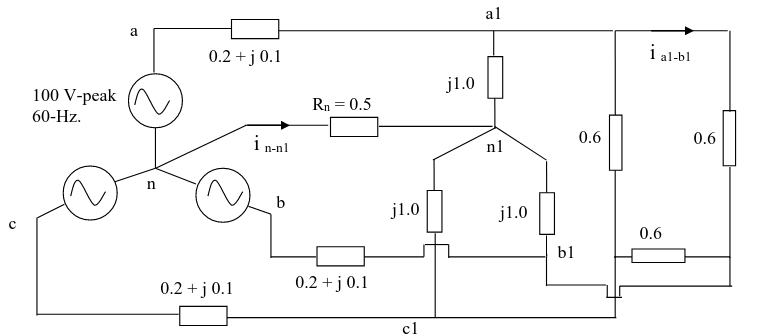
\includegraphics[width=\textwidth]{Figures/Lab\ Two/Diagram.png}
  \caption{Simulated Circuit}
  \label{fig:1}
\end{figure}

After simulating the circuit, data related to the voltage at various nodes and current through various loops was taken, most importantly nodes $a_1$ to $b_1$, and along the neutral line $n_1$ to $n$.

\section{Results \& Analysis} 

\subsection{Original Circuit}

The first step of the experiment is to plot the waveforms of $V_{a_1\to b_1}$, $I_{a_1\to b_1}$, and $I_{n\to n_1}$. The result is shown in Figure \ref{fig:2} below:

  \begin{figure}[H]
    \centering
    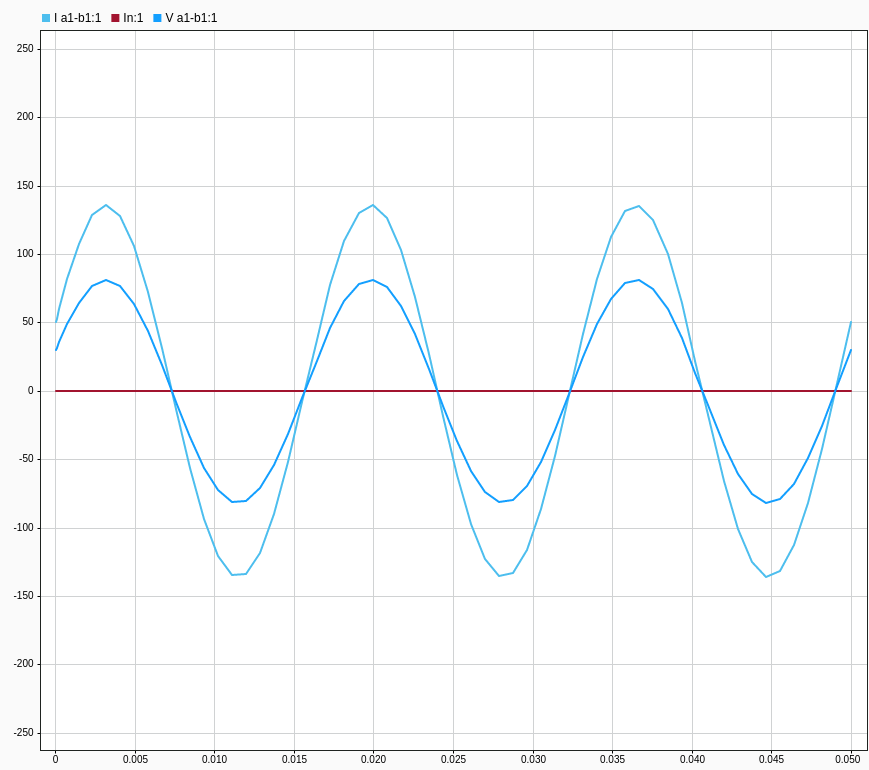
\includegraphics[width=.9\textwidth]{Figures/Lab\ Two/Parta.png}
    \caption{Waveforms for Part (a)}
    \label{fig:2}
  \end{figure}

  Here, we see the waveforms. Note that the neutral line has no current, as would be expected for a balanced circuit. From here, we construct a single phase equivalent circuit using Phase $a$. The circuit becomes:

  \begin{figure}[H]
    \centering
    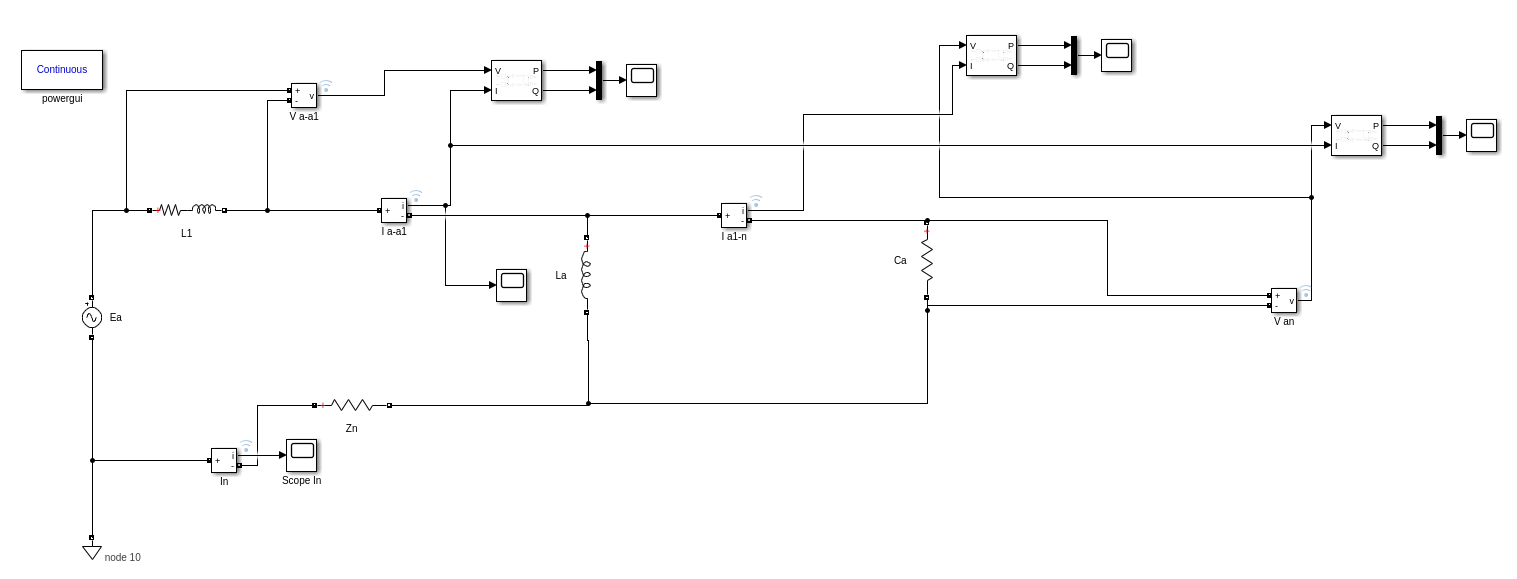
\includegraphics[width=.9\textwidth]{Figures/Lab\ Two/Partb.png}
    \caption{Single Phase Equivalent Circuit (Phase $a$)}
    \label{fig:3}
  \end{figure}

  Note that for the equivalent circuit, $C_a=.2[\si{\ohm}]$ instead of the original .6, since the configuration was in delta instead of 'Y' form.

\subsection{Modified Circuit}

Using the circuit to simulate, we may obtain the equivalent waveforms for $V_{a_1\to b_1}$ and $I_{a_1\to b_1}$:

\begin{figure}[H]
  \centering
  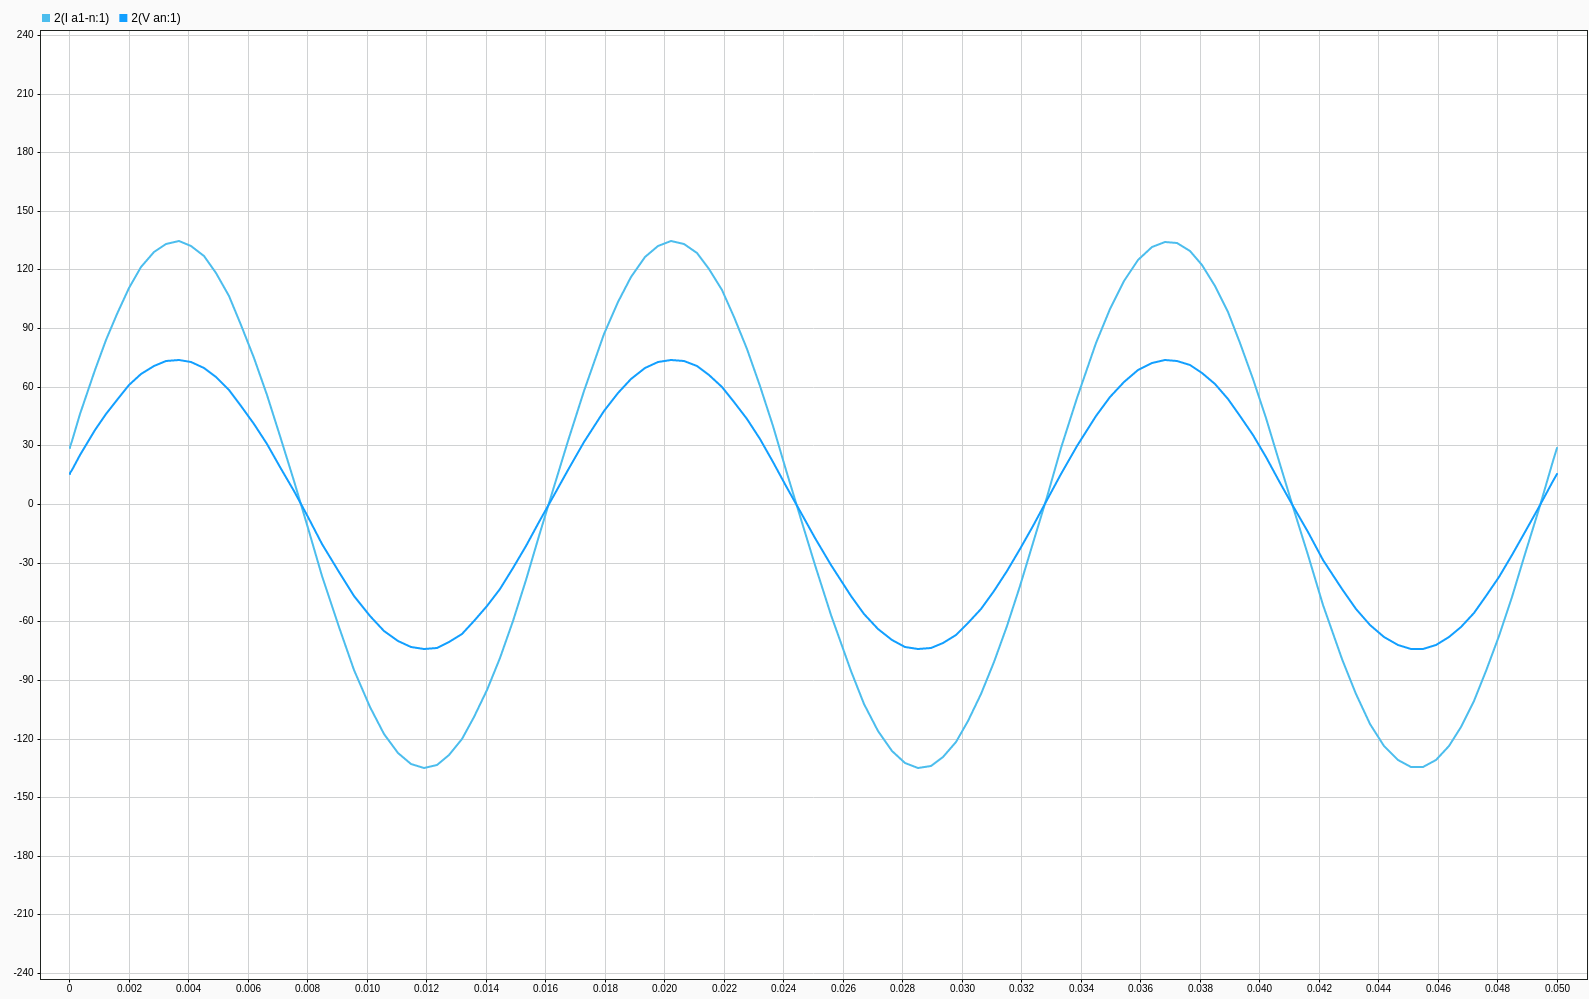
\includegraphics[width=.9\textwidth]{Figures/Lab\ Two/Partc.png}
  \caption{Waveforms Plotted Using Single-Phase Equivalent}
  \label{fig:4}
\end{figure}

Note that, as expected, the waveforms are equivalent to those shown in Figure \ref{fig:2}

\subsection{Changing the Neutral Line Impedance}

From here, we return to the original three-phase circuit, but now we modify the parameters. First, we change the neutral line impedance from $R_n=.5[\si{\ohm}]$ to $R_n=50[\si{\ohm}]$. Plotting the same waveforms, we get:

\begin{figure}[H]
  \centering
  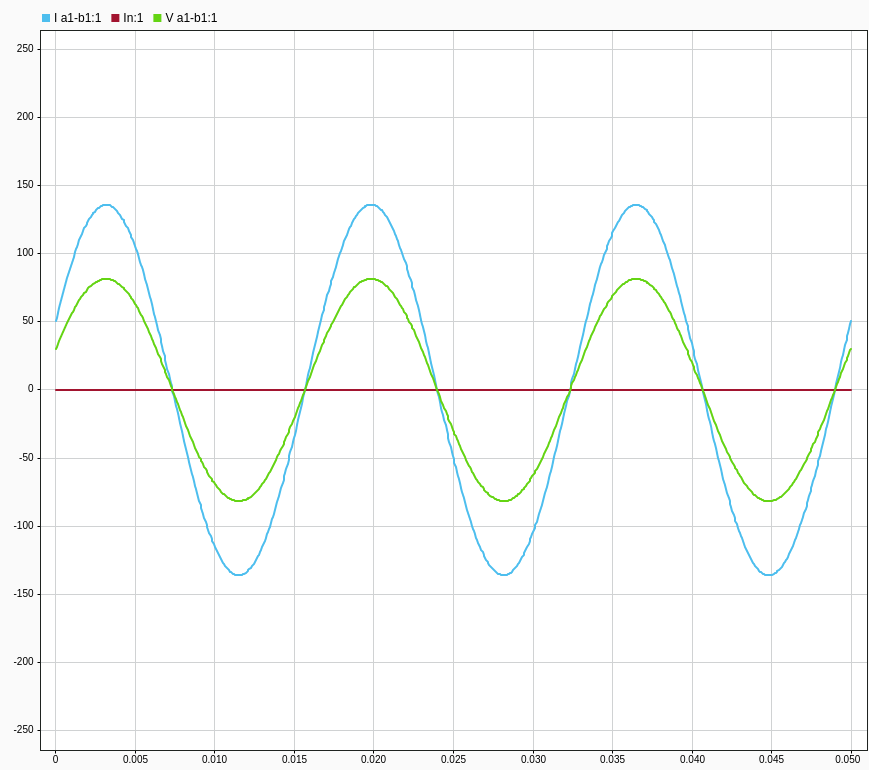
\includegraphics[width=.9\textwidth]{Figures/Lab\ Two/Partd.png}
  \caption{Waveforms with Changed Neutral Line Impedance}
  \label{fig:5}
\end{figure}

Once again, we see no change, as expected. This is because the neutral line still experiences no current flow, as the circuit remains balanced.

\subsection{Unbalancing the Circuit}

We now change the impedance from $a_1$ to $n_1$ by a factor of ten. This results in the following waveforms:

\begin{figure}[H]
  \centering
  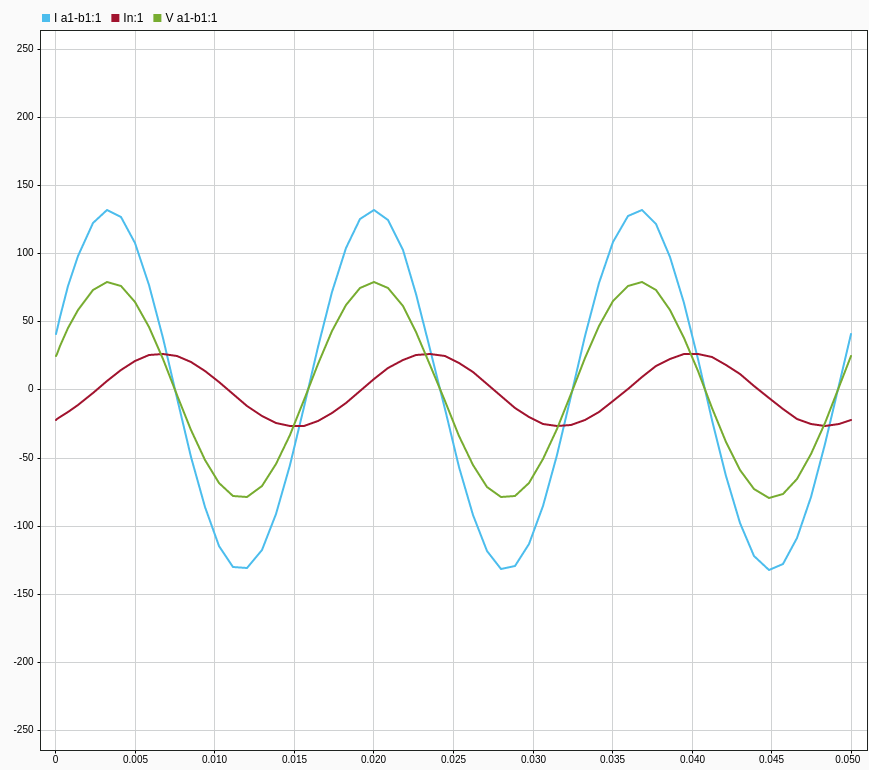
\includegraphics[width=.9\textwidth]{Figures/Lab\ Two/Parte.png}
  \caption{Waveforms for the Now-Unbalanced Circuit}
  \label{fig:6}
\end{figure}

We may notice with this waveform that, although the line-to-line difference remains the same, there is now a line-to-neutral difference. This causes current to flow through the neutral line, which can be seen by the red line.

\section{Conclusion}

Throughout this experiment, we verified several important concepts related to three-phase circuits. Namely, we confirmed that, for balanced three-phase circuits, a single-phase equivalent may be used to analyze each phase more easily. Additionally, we confirmed that current flows through the neutral line only in the unbalanced case.

\end{document}
